%%%%%%%%%%%%%%%%%%%%%%%%%% lecture-11
%\begin{frame}[shrink]
%  \frametitle{lecture-11 主要内容}
%  \framesubtitle{字符串处理库函数及程序举例}
%  %\tableofcontents[hideallsubsections]
%  \tableofcontents
%\end{frame}

\section{字符串处理函数\#include<string.h>}

\begin{frame}[shrink,fragile]{字符串处理函数\#include<string.h>}
\vspace{-0.2cm}
\begin{itemize}
	\item 使用字符串处理库函数, 必须包含头文件\#include<string.h>
	\item 要求字符串必须以`$\backslash$0'结尾
\end{itemize}
\vspace{-0.2cm}
\begin{lstlisting}
#include<stdio.h>
#include<string.h>
int main()
{
   char s1[81]="ab"; // 自动追加s1[2]='\0'
   char s2[81]="cdef"; // 自动追加s2[4]='\0'
   
   // 连接两个字符串, 结果被放入s1中, s1数组要足够大,能够容纳两个字符串连接后的长度+1, 多一个字符长度是留给'\0'使用
   strcat(s1,s2); 
   
   puts(s1); // abcdef, 最后一个字符是'\0'
   puts(s2); // cdef, s2保持不变, 最后一个字符是'\0'
   return 0;
}
\end{lstlisting}
\end{frame}

%\subsection{连接和复制字符串strcat(s1,s2); strcpy(s1,s2); strncpy(s1,s2,n)}

\begin{frame}[shrink,fragile]{\small{连接和复制字符串strcat(s1,s2); strcpy(s1,s2); strncpy(s1,s2,n)}}
\vspace{-0.3cm}
\begin{lstlisting}
   char s1[81]="ab"; // 自动追加s1[2]='\0'
   char s2[81]="cdef"; // 自动追加s2[4]='\0'
   // 连接两个字符串, 结果被放入s1中, s1数组要足够大,能够容纳两个字符串连接后的长度+1, 多一个字符长度是留给'\0'使用
   strcat(s1,s2); 
   puts(s1); // abcdef, 最后一个字符是'\0'
   puts(s2); // cdef, s2保持不变, 最后一个字符是'\0'
   // 把s2复制给s1, 因此s1数组也要足够大
   strcpy(s1,s2);  // s1=s2; 是错误的, 因为数组名表示地址常量
   puts(s1); // cdef, 最后一个字符是'\0'
   puts(s2); // cdef, s2保持不变, 最后一个字符是'\0'
   strncpy(s1,"1234",2); // 复制s2的前n个字符给s1,覆盖s1相应位置的字符, n要小于s1的数组长度
   puts(s1); // 12ef
\end{lstlisting}
\end{frame}

%\subsection{字符串比较strcmp(s1,s2); strncmp(s1,s2,n)}

\begin{frame}[shrink,fragile]{字符串比较strcmp(s1,s2); strncmp(s1,s2,n)}
\begin{lstlisting}
   char s1[81]="ab"; // 自动追加s1[2]='\0'
   char s2[81]="cdef"; // 自动追加s2[4]='\0'
   // 从左到右逐字符比较串s1和s2,大于返回1, 小于返回-1, 同时到达'\0'返回0表示相等
   printf("%d",strcmp(s1,s2)); // -1
   if(strcmp(s1,s2)==-1) printf("s1 < s2\n");
   printf("%d\n",strcmp("abad","ab1d")); // 1
   printf("%d\n",strcmp("1234","1234")); // 0
   printf("%d\n",strcmp("12","1234")); // -1
   printf("%d\n",strcmp("1234","12")); // 1  
   // 仅比较前n个字符
   printf("%d\n",strncmp("1234","12",2)); // 0
\end{lstlisting}
\end{frame}

%\subsection{获取字符串的长度strlen(s)}

\begin{frame}[shrink,fragile]{获取字符串的长度strlen(s)}
\begin{lstlisting}
   char s1[81]="ab"; // 自动追加s1[2]='\0'
   char s2[81]="cdef"; // 自动追加s2[4]='\0'
   int i;
   // 获取字符串的长度,不包括字符串结尾字符'\0'
   printf("%d,%d\n",strlen(s1), strlen(s2)); // 2,4
   for(i=0;i<strlen(s1);i++) printf("%c ",s[i]); // a b
   // 相当于下面程序段计算出的字符串长度len
   int len=0;
   for(i=0; s1[i]!='\0'; i++) len++;
   printf("\n字符串s1的长度=%d\n", len);
\end{lstlisting}
\end{frame}

%\subsection{大小写转换strlwr(s); strupr(s)}

\begin{frame}[shrink,fragile]{大小写转换strlwr(s); strupr(s)}
\begin{lstlisting}
char s1[81]="abCD12"; // 自动追加s1[2]='\0'
char s2[81]="cD12ef"; // 自动追加s2[4]='\0'
int i;
strlwr(s1); // 大写转小写
puts(s1); // abcd12
 
strupr(s2); // 小写转大写
puts(s2); // CD12EF

// 小写转大写, 等效于下面程序段
for(i=0;s2[i]!='\0';i++)
  if(s2[i]>='a' && s2[i]<='z') s2[i]-=32;  // s2[i]=s2[i]-32
\end{lstlisting}
\end{frame}

\section{程序举例}

%\subsection{统计单词数}

\begin{frame}[shrink,fragile]{\small{例6.8 输入一行字符, 统计其中有多少个单词, 单词之间用空格(可能多个)分隔开。}}
\vspace{-0.4cm}
\begin{tikzpicture}
\node[text width=1.0\textwidth] (t)
{
	\begin{lstlisting}
	// 定义变量
	char string[81]; // 用于存放字符串。
	int i; // 计数器,用于遍历字符串中的每个字符。
	int word=0; // 用于判断是否开始了一个新单词的标志。若word=0表示未出现新单词, 如出现了新单词, 就把word置成1。
	int num=0; //用于统计单词数。
	\end{lstlisting}
};

\node[text width=0.47\textwidth,anchor=north west] (t1) at($(t.south west)+(0.4cm,0.2cm)$) {
	 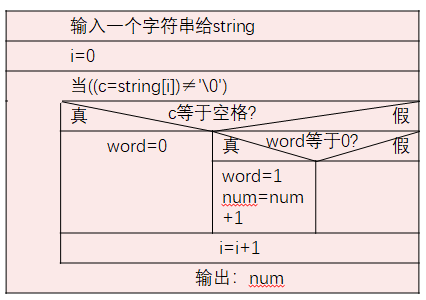
\includegraphics[scale=0.45]{ex6-8}
};

\node[anchor=west,text width=0.37\textwidth,fill=green,rounded corners] at(t1.east)
{
	$word=0; num=0; $
	
	\medskip
	
	$\underset{w=0}{\square}\overset{w=0}{\square}
	\underset{\underset{\underset{n++}{w=1}}{\downarrow}}{H}ow
	\overset{w=0}{\square}
	\underset{\underset{\underset{n++}{w=1}}{\downarrow}}{A}re
	\overset{w=0}{\square}
	\underset{\underset{\underset{n++}{w=1}}{\downarrow}}{Y}ou$
};
\end{tikzpicture}
\end{frame}

\begin{frame}[shrink,fragile]{\small{解: 例6.8 输入一行字符, 统计其中有多少个单词, 单词之间用空格(可能多个)分隔开。}}
\vspace{-0.4cm}
\begin{tikzpicture}
\node[text width=1.0\textwidth] (t)
{
\begin{lstlisting}
char string[81];
int i,num=0,word=0;
char c;
gets(string); //输入一个字符串给字符数组string
for(i=0;(c=string[i])!='\0';i++) //只要字符不是'\0'就循环,条件表达式:第i个字符赋值给c, 并且c$\ne$'\0'
{
   if(c==' ') word=0; //若是空格字符,使word置0
   else if(word==0) //如果不是空格字符且word原值为0
   { 
     word=1; //使word置1
     num++; //num累加1,表示增加一个单词
   }
}
printf("%d words in this line.\n",num); //输出单词数
\end{lstlisting}
};
\node[anchor=north east,text width=0.37\textwidth,fill=green,rounded corners] at($(t.north east)+(0,-0.3cm)$)
{
	$word=0; num=0;$
	
	\medskip
	
	$\underset{w=0}{\square}\overset{w=0}{\square}
	\underset{\underset{\underset{n++}{w=1}}{\downarrow}}{H}ow
	\overset{w=0}{\square}
	\underset{\underset{\underset{n++}{w=1}}{\downarrow}}{A}re
	\overset{w=0}{\square}
	\underset{\underset{\underset{n++}{w=1}}{\downarrow}}{Y}ou$
};
\end{tikzpicture}
\end{frame}

%\subsection{求多个字符串中的较大者}

\begin{frame}[shrink,fragile]{\small{例6.9 有3个字符串,要求找出其中``最大"者。}}
\pause
\begin{lstlisting}
char str[3][20]; //定义二维字符数组, 存放3个字符串。【重点学习】
char string[20]; //定义一维字符数组,作为交换字符串时的临时字符数组
int i;
for(i=0;i<3;i++)
   gets(str[i]); //读入3个字符串,分别给str[0],str[1],str[2]

if(strcmp(str[0],str[1])>0) //若str[0]大于str[1]
     strcpy(string,str[0]); //把str[0]的字符串赋给字符数组string
else //若str[0]小于等于str[1]
     strcpy(string,str[1]); //把str[1]的字符串赋给字符数组string 
if(strcmp(str[2],string)>0) //若str[2]大于string
     strcpy(string,str[2]); //把str[2]的字符串赋给字符数组string
printf("\nthe largest string is:\n%s\n",string); //输出string
\end{lstlisting}
\end{frame}


\begin{frame}[shrink,fragile]{\small{另解: 例6.9 有3个字符串,要求找出其中``最大"者。}}
\begin{lstlisting}
#include<stdio.h>
#include<string.h>
int main()                   
{  
   char s[20],max[20];  int i;
   for(i=0;i<3;i++)
   {
      if(i==0)gets(max); // 常用技巧: 初始, 第一个字符串就是最大者。
      else // 随后的字符串与max比较
      {
         gets(s);
         if(strcmp(s,max)>0) strcpy(max,s); // 如果该字符串比max大, 替换之。
      }
   }
   printf("\nthe largest string is:\n%s\n",max);
   return 0;           
}
\end{lstlisting}
\end{frame}  

%\subsection{矩阵乘法}

\begin{frame}[shrink,fragile]{例: 矩阵乘法}
\vspace{-0.4cm}
\begin{align*}
&c[M][N],a[M][P],b[P][N];\\ &c[i][j]=\sum_{k=0}^{P-1}a[i][k]b[k][j]=a[i][0]b[0][j]+a[i][1]b[1][j]+\cdots +a[i][P-1]b[P-1][j]
\end{align*}
\begin{scriptsize}
\begin{align*}
&a=\left[\begin{array}[l]{ccc}
a[0][0] & a[0][1] & a[0][2]\\
a[1][0] & a[1][1] & a[1][2]
\end{array}
\right]\quad
b=\left[\begin{array}[l]{ccc}
b[0][0] & b[0][1] \\
b[1][0] & b[1][1] \\
b[2][0] & b[2][1]
\end{array}
\right]\\
&c=\left[\begin{array}[l]{ccc}
a[0][0]b[0][0]+a[0][1]b[1][0]+a[0][2]b[2][0] & a[0][0]b[0][1]+a[0][1]b[1][1]+a[0][2]b[2][1] \\
a[1][0]b[0][0]+a[1][1]b[1][0]+a[1][2]b[2][0] & a[1][0]b[0][1]+a[1][1]b[1][1]+a[1][2]b[2][1]
\end{array}
\right]
\end{align*}
\end{scriptsize}
\\
%\vspace{0.2cm}
%\medskip
\pause
\bigskip
\textbf{\textcolor{blue}{c[i][j]=a的第i行各列(k)和b的第j列各行(k)的乘积累加. $k=0\to(P-1)$}}
\end{frame}

\begin{frame}[shrink,fragile]{解: 矩阵乘法}
\begin{lstlisting}
#define M 100 // 估计的最大值
#define P 50
#define N 100 
int c[M][N],a[M][P]={{1,2,4}},b[P][N]={{2,1,3},{7,9,10},{5,7,1}}; // c={36,47,27}
int m=4,n=2,p=3; // M,N,P实际大小
int i,j,k; //i,j,k分别是m,n,p的循环变量 
for(i=0;i<m;i++) 
{
   for(j=0;j<n;j++)
   {
     c[i][j]=0;
     for(k=0;k<p;k++) 
        c[i][j]+=a[i][k]*b[k][j]; // a的第i行各列(k)和b的第j列各行(k)的乘积累加 
     printf("c[%d][%d]=%d\n",i,j,c[i][j]); // 输出测试
   }
}
\end{lstlisting}
\end{frame}

\begin{frame}[shrink,fragile]
\small{曾经的测试用例}
\begin{lstlisting}
//int c[M][N],a[M][P]={{1,2,4}},b[P][N]={{2,1,3},{7,9,10},{5,7,1}}; // c={36,47,27}
//int m=1,n=3,p=3; // M,N,P实际大小
//int c[M][N],a[M][P]={{2,1},{4,3}},b[P][N]={{1,2},{1,0}}; // c={{3,4},{7,8}}
//int m=2,n=2,p=2; // M,N,P实际大小
//int c[M][N],a[M][P]={{1,0,2},{-1,3,1}},b[P][N]={{3,1},{2,1},{1,0}}; // c={{5,1},{4,2}}
//int m=2,n=2,p=3; // M,N,P实际大小
int c[M][N],a[M][P]={{5,2,4},{3,8,2},{6,0,4},{0,1,6}},b[P][N]={{2,4},{1,3},{3,2}}; // c={{24,34},{20,40},{24,32},{19,15}}
int m=4,n=2,p=3; // M,N,P实际大小
int i,j,k; //i,j,k分别是m,n,p的循环变量  
// 添加输入语句
scanf("%d%d%d\n", &m,&n,&p);
for(i=0;i<m;i++)
  for(k=0;k<p;k++) scanf("%d",&a[i][k]);
for(k=0;k<p;k++)
  for(j=0;j<n;j++) scanf("%d",&b[k][j]);
...
\end{lstlisting}
\end{frame}  

%\begin{frame}[shrink]
%\frametitle{lecture-12 主要内容}
%\framesubtitle{字符串处理库函数及程序举例}
%%\tableofcontents[hideallsubsections]
%\tableofcontents
%\end{frame}               






